\section{Ziel}
Ziel ist es die elastische Konstante Torsionsmodul $G$ einer Metallegierung, sowie das magnetische Moment eines Permanentmagneten zu bestimmen.


\section{Vorbereitung}
\subsection{Elastizitätstheorie}
Wirkt eine Kraft auf eine Fläche, so führt dies unter anderem zu einer Gestalts- und Volumenänderung.
Dabei unterscheidet man in der Mechanik, unter folgenden Kräften:
\begin{description}
    \item[]
    Kräften, die an jedem Volumenelement angreifen, wie der Schwerkraft, die zur Translation bzw. Rotation führen.
    \item[]
    Kräften, die an jedem Oberflächenelement angreifen, bewirken Gestalts- und Volumenänderungen.
\end{description}

Wirkt die Kraft senkrecht zu Oberfläche so spricht man von der Normalspannung $\sigma$ bzw. Druck $p$ oder parallel zur Oberfläche,
dann spricht man von der Tangential- bzw Schubspannung $\tau$.
\begin{figure}[h]
  \centering
  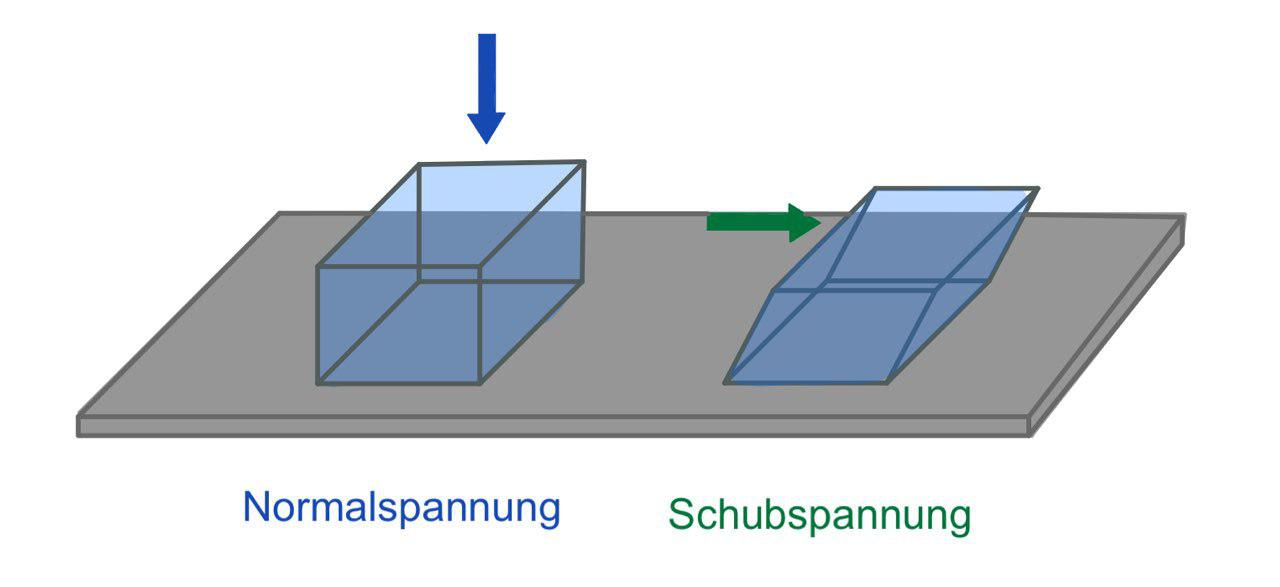
\includegraphics[width=0.4\textwidth, height=0.2\textwidth]{bilder/Spannungkomponenten.jpg}
  \caption{Spannungskomponenten}
  \label{fig:Spannungkomponenten}
\end{figure}

Geschieht diese Krafteinwirkung im elastischen Bereich des Materials,
so bilden die elastischen Konstanten den Proportionalitätsfaktor zwischen der
wirkenden Spannung und der Deformation.\\
Man spricht hierbei vom Hookschen Gesetz \ref{sec:Hooksche_Gesetz}.

\subsection{Das Hooksche Gesetz}
\label{sec:Hooksche_Gesetz}
Bewirkt die Spannung beim Material eine elastische Verformung, so kehrt dieser, nach dem Einwirken 
der Kraft wieder in seine Ausgangsform zurück (reversibler Vorgang). Man nennt diesen Bereich, elastischen bzw. hookschen Bereich.
Dabei gilt:
\begin{align}
    \sigma &= E \; \frac{\Delta L}{L} & \mathrm{bzw.} & & P &=Q \;\frac{\Delta V}{V}
\end{align}
\label{eqn:def_hooksche}
\newpage

\subsection{Symmetrien}
Ein vollständiges Hooksches Gesetz zu formulieren, ist dabei nicht auf die einfach dagelegte From wie 
in Gleichung \eqref{eqn:def_hooksche} beschränkt.
Denn eine niedrige Symmetrie des Materials führt zu richtungsabbhängigen Kräften, welche mehr Konstanten
benögtigen, um die Deformation vollständig zu beschrieben.
3 Konstanten für die jeweilige Gestalts-, die Volumenelastizität und 6 Konstanten für die Deformation,
führen somit auf eine 6x6- Matrix, also insgesamt 36 Konstanten.\newline
Diese Vielzahl an Konstanten, kann durch Materialsymmetrien (z.\;B. Energieprinzip) verringert werden.




\subsection{Elastische Konstanten isotroper Stoffe}
In der Praxis haben sich für isotrope Stoffe vier Elastische Konstanten durchgesetzt.\\
\begin{description}
\item[Elastizitätsmodul $E$:]
    Das Elastizitätsmodul $E$ beschreibt die relative Längenänderung in Spannungsrichtung
    bei einer wirkenden Normalspannung $\sigma$.
    \begin{equation}
        \sigma = E \; \frac{\Delta L}{L}
        \label{eqn:def_elastizitätsmodul}
    \end{equation}

\item[Schubmodul,Torsionsmodul $G$:]
    Das Schub- bzw. Torsionmodul $G$ beschreibt die Gestaltselastizität bei einer
    wirkenden Schubspannung $\tau$
    \begin{equation}
        \tau = G \; \alpha
        \label{eqn:def_schubmodul}
    \end{equation}
    
    \begin{figure}[h]
        \centering
        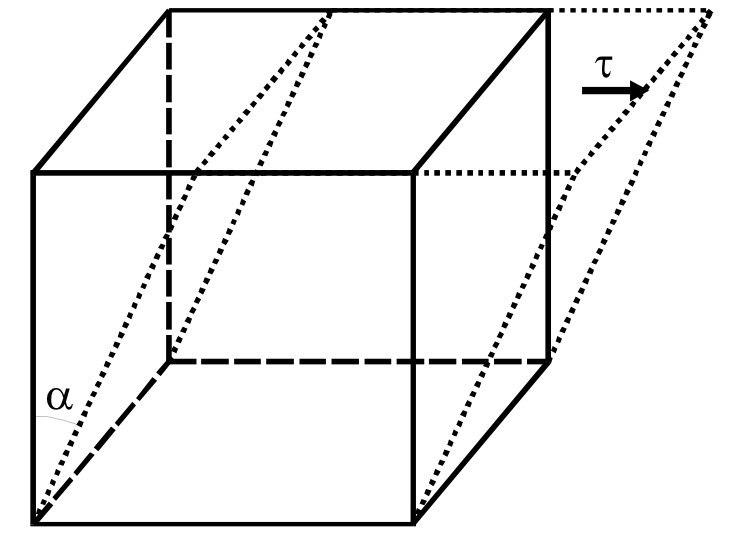
\includegraphics[width=0.3\textwidth, height=0.2\textwidth]{bilder/Schubmodul.jpg}
        \caption{Schubmodul $G$,\cite[4]{Anleitung}}        
        \label{fig:schubmodul}
    \end{figure}

\item[Kompressionsmodul $Q$:]
    Das Kompressionsmodul $Q$ beschreibt die Volumenelastizität.

\newpage
\item[Poissonsche Querkontraktionszahl $\mu$:]
    Die Poissonsche Querkontroationszahl $\mu$ beschreibt die Längenänderung durch die Normalspannung $\sigma$
    senkrecht zu Richung von $\sigma$.
    \begin{equation}
        \mu := -\frac{\Delta B}{B} \cdot \frac{L}{\Delta L}
        \label{eqn:def_poissonsche}
    \end{equation}
    
    \begin{figure}[h]
        \centering
        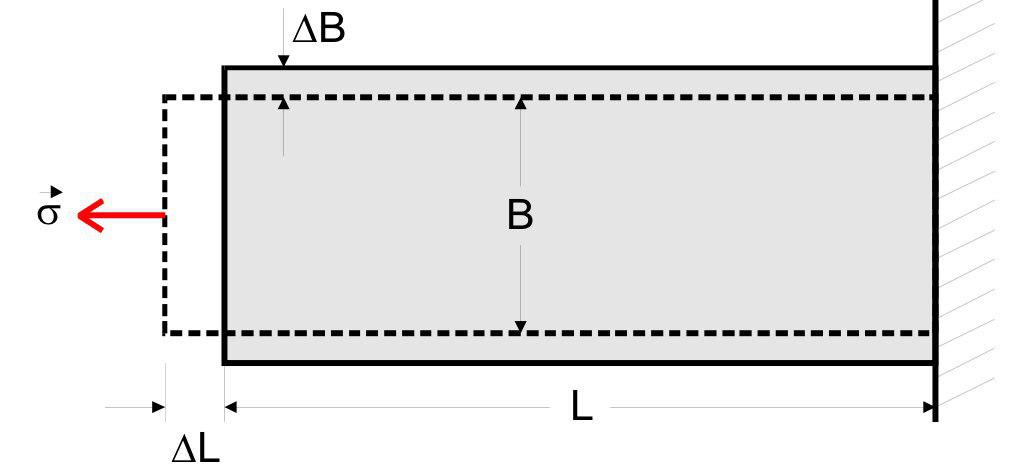
\includegraphics[width=0.35\textwidth, height=0.15\textwidth]{bilder/Poissonsche_Quer.jpg}
        \caption{Poissonsche Querkontraktionszahl $\mu$,\cite[3]{Anleitung}}        
        \label{fig:poissonsche_Quer}
    \end{figure}
\end{description}


Dabei sind die vier Konstanten $G$, $E$, $Q$ und $\mu$ nicht unabhängig von einander.
Es gilt folgende Beziehung:
\begin{gather}
    E = 2\;G\;(\mu\,+\,1) \\
    E = 3\;(1\;-2\mu)\;Q
    \label{eqn:Beziehung}
\end{gather}


\subsection{Problematik: Elastisches Nachwirken}
%!!! Hier MUSS zitiert werden!
Das Elastische Nachwirken ist eine Eigenschaft von Materialien, die nicht augenblicklich die Lage ihres definitiven 
Gleichgwichts annhemen, sondern im Laufe der Zeit bei fortdauernden wirkenden äußeren Kräften noch weiter Änderungen zu
erfahren und nachdem die äußern Kräfte zu wirken aufgehört haben, nicht sofort, sondern erst nach einiger Zeit in den 
ursprünglichen Zustand wieder zurückzukehren.\cite{elastisches_Nachwirken}
Dies gilt besonders bei Materialien mit niedrigen Schmelztemperaturen.\\
Dies führ zu großen Fehlerquellen bei Versuch die elastischen Konstanten direkt statisch 
zu messen.\newline
Um diese Fehlerquelle zu minimieren, verwende man dynamische Methoden (s. Kapitel: \ref{sec:Durchfuehrung}).
\label{sec:nachwirken_vorb}


\label{sec:Theorie}
